\documentclass[twoside, 12pt]{article}
\usepackage{amsmath}
\usepackage{graphicx, xdipp, url, fancyvrb}
\usepackage[hidelinks]{hyperref}
\cestina
\usepackage{listings}
\lstset{
  basicstyle=\ttfamily\small,
  breaklines=true,
  frame=single,
  numbers=left,
  numberstyle=\tiny,
  language=Python
}
\usepackage{caption}
\usepackage{amssymb}
\usepackage{booktabs}
\usepackage{float}

\begin{document}

\makeatletter
\def\typprace{Semestrální}
\def\c@prace{projekt}
\def\a@prace{project}
\makeatother
\titul{Klasifikace sentimentu, shlukování témat a vyhledávání podobných hotelových recenzí}
{\begin{tabular}[b]{@{}r} Bc. Jan Dub \\ Bc. David Krčmář \end{tabular}}{doc. Ing. František Dařena, Ph.D.}{Brno 2026}

\abstract{Dub, J.; Krčmář, D. Sentiment Classification, Topic Clustering and Similarity Search in Hotel Reviews. Semester project. Mendel University in Brno, 2026.}
{This semester project presents a compact end-to-end text-mining pipeline for hotel reviews from the Kaggle dataset \emph{515K Hotel Reviews Data in Europe}. The work validates and summarizes the original CSV file, preprocesses review text, trains and compares three classical classifiers, evaluates chi-square feature selection, clusters negative reviews with K-Means, and builds a TF-IDF retrieval module with cosine similarity. The dataset contains 515,738 reviews and 17 columns. On a 50,000-review development sample, the best sentiment configuration combines \textbf{TF-IDF with unigrams and bigrams, \texttt{SelectKBest(chi2, k=5000)} and Linear SVM}, reaching \textbf{macro F1 = 0.8120} and \textbf{accuracy = 95.03\%}. Negative-review clustering is interpretable but only weakly separated, with the best result at \textbf{k = 7} and \textbf{silhouette score = 0.0100}. Retrieval works well for specific multi-word queries and degrades for generic queries. The report discusses both the practical usefulness and the limits of classical text-mining methods on noisy user-generated review data.}

\abstrakt{Dub, J.; Krčmář, D. Klasifikace sentimentu, shlukování témat a vyhledávání podobných hotelových recenzí. Semestrální projekt. Mendelova univerzita v Brně, 2026.}
{Tento semestrální projekt představuje kompaktní end-to-end text-mining pipeline nad hotelovými recenzemi z Kaggle datasetu \emph{515K Hotel Reviews Data in Europe}. Práce ověřuje a shrnuje původní CSV soubor, předzpracovává text recenzí, trénuje a porovnává tři klasické klasifikační modely, vyhodnocuje výběr atributů pomocí chi-kvadrát testu, shlukuje negativní recenze metodou K-Means a buduje retrieval modul založený na TF-IDF a cosine similarity. Dataset obsahuje 515\,738 recenzí a 17 sloupců. Na development vzorku o velikosti 50\,000 recenzí dosáhla nejlepší konfigurace sentiment klasifikace ve složení \textbf{TF-IDF s unigramy a bigramy, \texttt{SelectKBest(chi2, k=5000)} a Linear SVM} hodnot \textbf{macro F1 = 0{,}8120} a \textbf{accuracy = 95{,}03~\%}. Clustering negativních recenzí je interpretovatelný, ale jen slabě separovaný; nejlepší konfigurace vyšla pro \textbf{k = 7} se \textbf{silhouette score = 0{,}0100}. Retrieval funguje dobře pro konkrétní víceslovné dotazy a ztrácí kvalitu u obecných formulací. Report diskutuje praktický přínos i limity klasických text-mining metod na hlučných uživatelských recenzích.}

\keywords{text mining, hotel reviews, sentiment classification, clustering, information retrieval, TF-IDF, Linear SVM}
\klslova{text mining, hotelové recenze, klasifikace sentimentu, clustering, information retrieval, TF-IDF, Linear SVM}

\obsah

\section*{\LARGE\textbf{Seznam použitých pojmů}}

\begin{itemize}
    \item \textbf{\textit{TF-IDF}}: vážená reprezentace textu, která zvýrazňuje termy důležité pro konkrétní dokument a potlačuje příliš častá slova v celé kolekci.
    \item \textbf{\textit{n-gram}}: posloupnost $n$ tokenů; v této práci porovnáváme unigramy a kombinaci unigramů s bigramy.
    \item \textbf{\textit{Linear SVM}}: lineární Support Vector Machine, tedy klasifikátor vhodný pro řídké textové reprezentace s vysokým počtem atributů.
    \item \textbf{\textit{Chi-square feature selection}}: metoda výběru atributů podle závislosti mezi termem a cílovou třídou.
    \item \textbf{\textit{K-Means}}: clustering algoritmus, který rozděluje dokumenty do předem zadaného počtu clusterů podle vzdálenosti od centroidů.
    \item \textbf{\textit{Silhouette score}}: interní metrika clusteringu hodnotící kompaktnost clusteru a jeho oddělení od ostatních clusterů.
    \item \textbf{\textit{Cosine similarity}}: míra podobnosti dvou vektorů podle úhlu mezi nimi; standardní volba pro porovnávání TF-IDF reprezentací.
\end{itemize}

\kapitola{Úvod a motivace}

Hotelové recenze jsou vhodným příkladem reálných textových dat, na nichž lze ukázat hlavní úlohy text miningu v jedné společné pipeline. Každá recenze kombinuje volný text, číselné skóre a doplňující metadata. Tato kombinace umožňuje současně řešit klasifikaci sentimentu, tematické shlukování i vyhledávání podobných dokumentů.

Praktická motivace je dvojí. Zaprvé hotelové recenze představují obchodně důležitý zdroj zpětné vazby pro provozovatele ubytování i agregátory typu Booking.com. Zadruhé jde o dataset s realistickým množstvím šumu: obsahuje placeholdery typu \texttt{No Negative}, velmi krátké zápisy, různou délku recenzí i nevyvážené rozdělení výsledných tříd. Projekt je proto vhodný nejen pro demonstraci funkčních metod, ale i pro otevřenou diskusi jejich limitů.

Z pohledu předmětu práce pokrývá reprezentaci textu, preprocessing, klasifikaci, feature selection, clustering i information retrieval. Místo jedné izolované úlohy tak vzniká konzistentní text-mining projekt se sdíleným datasetovým základem a společným vyhodnocením.

\kapitola{Cíl práce a výzkumné otázky}

Cílem práce je navrhnout a implementovat kompaktní text-mining pipeline pro analýzu hotelových recenzí a ověřit, které klasické metody fungují na tomto typu dat nejlépe.

\sekce{Hlavní cíle}

\begin{enumerate}
    \item připravit a zdokumentovat dataset hotelových recenzí,
    \item vytvořit společnou textovou reprezentaci vhodnou pro strojové učení,
    \item natrénovat a porovnat několik modelů sentiment klasifikace,
    \item vyhodnotit vliv výběru atributů pomocí \texttt{SelectKBest(chi2)},
    \item identifikovat hlavní tematické okruhy v negativních recenzích pomocí clusteringu,
    \item vytvořit jednoduchý retrieval modul vracející podobné recenze pro zadaný dotaz.
\end{enumerate}

\sekce{Výzkumné otázky}

\begin{enumerate}
    \item Který ze tří klasických modelů (\texttt{MultinomialNB}, \texttt{LogisticRegression}, \texttt{LinearSVC}) dosahuje na hotelových recenzích nejlepší kvality?
    \item Pomůže výběr atributů pomocí \texttt{SelectKBest(chi2)} oproti čistému TF-IDF baseline?
    \item Jaká témata dominují negativním recenzím a nakolik jsou výsledné clustery interpretovatelné?
    \item Nakolik dobře funguje retrieval založený na TF-IDF a cosine similarity pro konkrétní a obecné dotazy?
\end{enumerate}

\kapitola{Dataset}

\sekce{Zdroj a struktura dat}

Primárním zdrojem je Kaggle dataset \emph{515K Hotel Reviews Data in Europe} od Jiashena Liu. Pracujeme s originálním souborem \texttt{Hotel\_Reviews.csv}, který je uložen v lokální struktuře projektu v adresáři \texttt{data/raw/}. Dataset obsahuje textová pole \texttt{Positive\_Review} a \texttt{Negative\_Review}, dále číselné skóre \texttt{Reviewer\_Score} a pomocná metadata, například \texttt{Hotel\_Name}, \texttt{Average\_Score}, \texttt{Tags} nebo zeměpisnou polohu hotelu.

\begin{table}[H]
\centering
\caption{Základní charakteristika datasetu}
\begin{tabular}{|p{5.2cm}|p{8cm}|}
\hline
\textbf{Položka} & \textbf{Hodnota} \\ \hline
Zdroj & Kaggle: \emph{515K Hotel Reviews Data in Europe} \\ \hline
Hlavní soubor & \texttt{Hotel\_Reviews.csv} \\ \hline
Počet řádků & 515\,738 \\ \hline
Počet sloupců & 17 \\ \hline
Klíčové atributy & \texttt{Positive\_Review}, \texttt{Negative\_Review}, \texttt{Reviewer\_Score}, \texttt{Hotel\_Name}, \texttt{Tags} \\ \hline
Datové typy & textová pole typu object, skóre typu float64, některé počty typu int64 \\ \hline
Chybějící hodnoty & v textových polích a skóre 0; u \texttt{lat}/\texttt{lng} celkem 3\,268 hodnot \\ \hline
Rozsah \texttt{Reviewer\_Score} & 2.5 až 10.0 \\ \hline
Průměr / medián skóre & 8.3951 / 8.8 \\ \hline
\end{tabular}
\end{table}

\sekce{Kvalita dat a praktická omezení}

Dataset je rozsáhlý, ale nikoli čistý. Velká část recenzí používá placeholdery typu \texttt{No Negative} nebo \texttt{No Positive}. V ověřeném lokálním snapshotu se vyskytuje 152\,663 hodnot typu \texttt{No Negative} a 37\,791 hodnot typu \texttt{No Positive}. Kromě toho se objevují i krátké pseudo-negativní výrazy jako \texttt{No complaints}, \texttt{Everything was perfect} nebo pouze \texttt{Breakfast}, které nejsou technicky placeholder, ale obsahově komplikují další zpracování.

Dalším omezením je výrazně pozitivní rozdělení skóre. Nejčastější hodnota v celém datasetu je 10.0, která se vyskytuje 115\,853krát, zatímco spodní část škály je zastoupena podstatně méně. To je důležité pro návrh labelů i pro interpretaci accuracy, která sama o sobě nestačí.

\sekce{Rozdělení skóre recenzí}

Rozdělení \texttt{Reviewer\_Score} ukazuje obrázek \ref{fig:score-distribution}. Vysoká koncentrace hodnocení v intervalu 8.3 až 10.0 potvrzuje, že jde o dataset s přirozeným pozitivním biasem.

\begin{figure}[H]
\centering
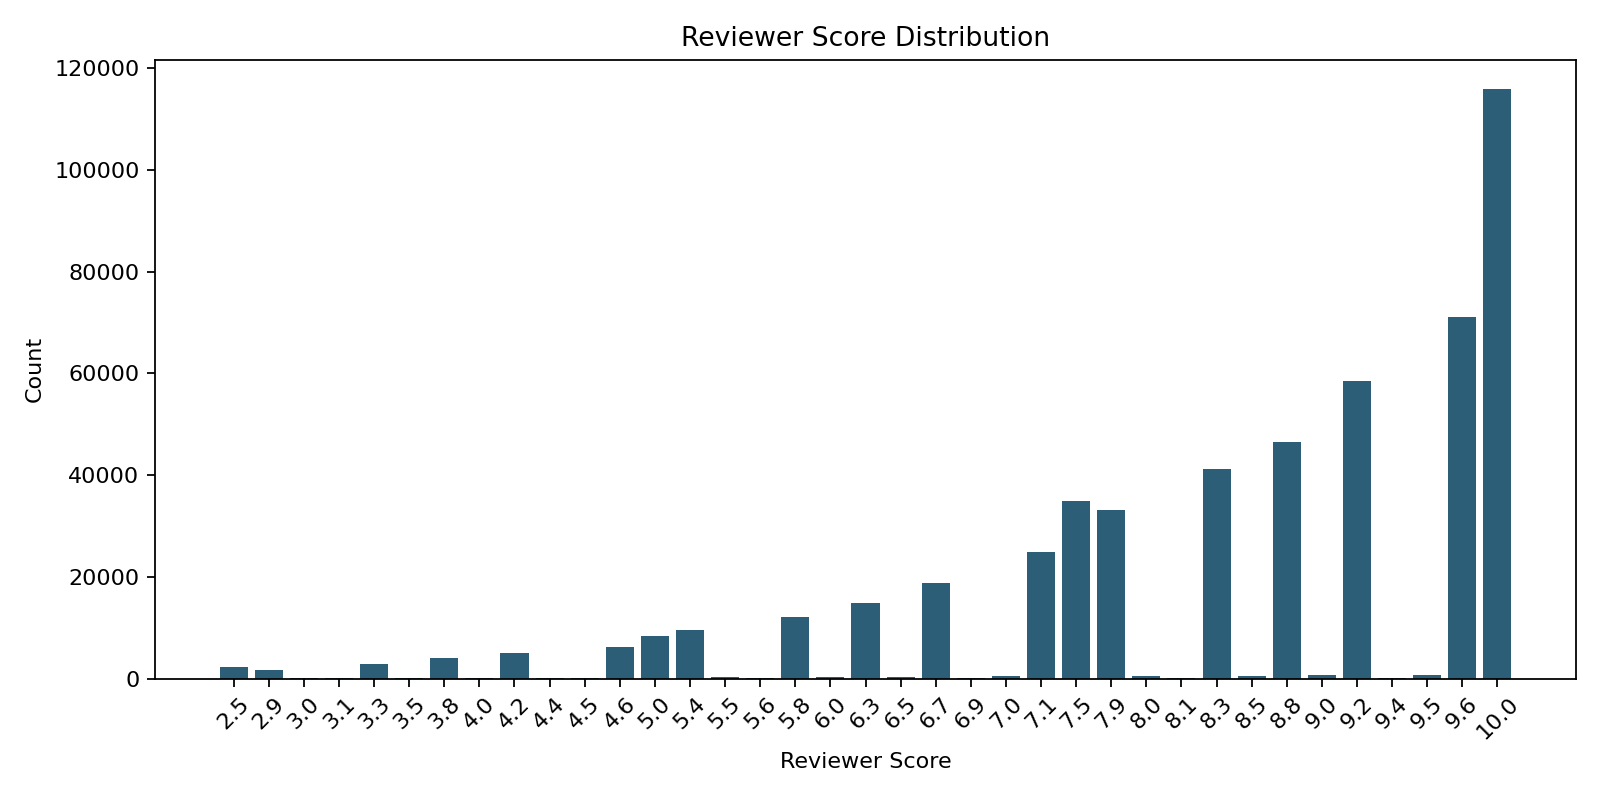
\includegraphics[width=0.95\textwidth]{outputs/visuals/reviewer_score_distribution.png}
\caption{Rozdělení hodnot \texttt{Reviewer\_Score} v celém datasetu}
\label{fig:score-distribution}
\end{figure}

\sekce{Pracovní režim}

Pro samotné experimenty jsme nepoužívali plný dataset ve všech krocích. Pro rychlé iterace a ladění se ukázal jako praktický vzorek 20\,000 až 50\,000 záznamů, zatímco plný dataset zůstává vhodný spíše jako volitelný benchmark. Tento kompromis odpovídá školnímu charakteru projektu: hlavním cílem je porovnání metod a interpretace výsledků, nikoli maximalizace výkonu za cenu dlouhých běhů a vyšších paměťových nároků.

\kapitola{Data preprocessing}

\sekce{Tvorba textových atributů}

V projektu vytváříme tři společné textové varianty:

\begin{itemize}
    \item \texttt{review\_text}: spojení pozitivní a negativní části recenze,
    \item \texttt{negative\_text}: pouze negativní část recenze,
    \item \texttt{positive\_text}: pouze pozitivní část recenze.
\end{itemize}

Pro sentiment klasifikaci se jako nejlepší volba ukázalo \texttt{review\_text}, protože kombinuje oba póly recenze a dává modelu nejvíce kontextu. Pro clustering jsme naopak používali \texttt{negative\_text}, kde jsou témata problémů čitelnější.

\sekce{Čisticí pipeline}

Před samotnou reprezentací proběhly následující kroky:

\begin{enumerate}
    \item náhrada placeholderů v polích \texttt{Positive\_Review} a \texttt{Negative\_Review} prázdným textem,
    \item odstranění prázdných vybraných textových polí,
    \item převod na malá písmena,
    \item odstranění nealfabetických znaků,
    \item normalizace mezer,
    \item odstranění záznamů, které zůstaly prázdné i po cleaningu.
\end{enumerate}

Na development vzorku o velikosti 50\,000 řádků vedl binární label filter a preprocessing k následujícímu průchodu daty:

\begin{table}[H]
\centering
\caption{Průchod daty po labelingu a preprocessingu}
\begin{tabular}{|p{7cm}|r|}
\hline
\textbf{Krok} & \textbf{Počet řádků} \\ \hline
Načtený development sample & 50\,000 \\ \hline
Po binárním labelingu & 35\,553 \\ \hline
Po odfiltrování prázdného textového pole & 35\,520 \\ \hline
Po final cleaningu & 35\,519 \\ \hline
Train split & 28\,415 \\ \hline
Test split & 7\,104 \\ \hline
\end{tabular}
\end{table}

\sekce{Reprezentace textu a labely}

Finální baseline pro klasifikaci používá TF-IDF reprezentaci z knihovny scikit-learn. Testovali jsme unigramy i kombinaci unigramů s bigramy; lepší se ukázala druhá varianta. Zvolená konfigurace byla:

\begin{itemize}
    \item \texttt{ngram\_range = (1, 2)},
    \item \texttt{min\_df = 5},
    \item \texttt{max\_df = 0.9},
    \item \texttt{max\_features = 50000},
    \item anglický seznam stop slov ze scikit-learn.
\end{itemize}

Sentiment labely byly vytvořeny binárně:

\begin{itemize}
    \item \texttt{Reviewer\_Score <= 5.0} $\rightarrow$ negative,
    \item \texttt{Reviewer\_Score >= 8.0} $\rightarrow$ positive,
    \item střední pásmo bylo z klasifikace vynecháno.
\end{itemize}

Tento návrh záměrně zvyšuje separaci tříd, ale zároveň zmenšuje datovou základnu. Po filtrování zůstalo na development vzorku 32\,502 pozitivních a 3\,017 negativních recenzí, což potvrzuje výraznou nevyváženost tříd.

\kapitola{Sentiment classification}

\sekce{Použité modely a evaluační nastavení}

Porovnávali jsme tři klasické modely vhodné pro řídké textové reprezentace:

\begin{itemize}
    \item \texttt{Multinomial Naive Bayes},
    \item \texttt{Logistic Regression},
    \item \texttt{Linear SVM}.
\end{itemize}

Pro rozdělení dat byl použit stratifikovaný train/test split v poměru 80/20. Kvůli nevyváženosti tříd sledujeme kromě accuracy také macro precision, macro recall a macro F1. To je důležité zejména proto, že vysoká accuracy může vznikat i při systematickém zanedbávání menšinové negativní třídy.

\sekce{Baseline výsledky bez feature selection}

Tabulka \ref{tab:classification-baseline} shrnuje výsledky baseline konfigurace nad \texttt{review\_text} s TF-IDF unigramy a bigramy.

\begin{table}[H]
\centering
\caption{Výsledky sentiment klasifikace bez feature selection}
\label{tab:classification-baseline}
\small
\begin{tabular}{|p{4.0cm}|c|c|c|c|}
\hline
\textbf{Model} & \textbf{Macro prec.} & \textbf{Macro rec.} & \textbf{Macro F1} & \textbf{Acc.} \\ \hline
Linear SVM & 0.8717 & 0.7602 & 0.8039 & 0.9481 \\ \hline
Logistic Regression & 0.9152 & 0.6982 & 0.7612 & 0.9447 \\ \hline
Multinomial Naive Bayes & 0.9476 & 0.5926 & 0.6374 & 0.9303 \\ \hline
\end{tabular}
\normalsize
\end{table}

Linear SVM skončil v baseline první. Logistic Regression zůstává konkurenceschopná, ale zaostává hlavně v macro recall. Naive Bayes sice drží slušnou accuracy, avšak na minoritní negativní třídě ztrácí, což se projeví výrazně slabším macro F1.

\sekce{Interpretace nejlepší baseline}

Pro nejlepší baseline model (\texttt{Linear SVM}) ukazuje confusion matrix následující chování:

\begin{table}[H]
\centering
\caption{Confusion matrix pro baseline Linear SVM}
\begin{tabular}{|l|c|c|}
\hline
\textbf{Skutečná / predikovaná třída} & \textbf{Negative} & \textbf{Positive} \\ \hline
Negative & 321 & 281 \\ \hline
Positive & 88 & 6\,413 \\ \hline
\end{tabular}
\end{table}

Model tedy velmi dobře rozpoznává pozitivní recenze, ale část negativních recenzí stále přiřazuje do pozitivní třídy. To odpovídá charakteru dat: negativní třída je menší, lexikálně méně homogenní a častěji obsahuje krátké či smíšené formulace.

\kapitola{Feature selection}

\sekce{Metoda a experimentální nastavení}

V další fázi jsme nad stejnou TF-IDF reprezentací aplikovali \texttt{SelectKBest(chi2)}. Cílem bylo ověřit, zda výběr atributů dokáže odstranit část šumu, zlepšit generalizaci a zároveň nabídnout lépe interpretovatelné termy pro sentiment.

Testovali jsme hodnoty $k \in \{0, 5000, 10000, 20000, 30000\}$, kde $k = 0$ znamená baseline bez feature selection. U vyšších hodnot se ukázalo, že skutečný počet aktivních atributů po vektorizaci je pouze 15\,266; proto konfigurace s $k = 20000$ a $k = 30000$ fakticky vracejí všechny atributy a reprodukují baseline.

\sekce{Porovnání konfigurací}

\begin{table}[H]
\centering
\caption{Vliv feature selection na nejlepší model (Linear SVM)}
\begin{tabular}{|c|c|c|}
\hline
\textbf{k} & \textbf{Macro F1} & \textbf{Accuracy} \\ \hline
0 & 0.8039 & 0.9481 \\ \hline
5\,000 & 0.8120 & 0.9503 \\ \hline
10\,000 & 0.8032 & 0.9479 \\ \hline
20\,000 & 0.8039 & 0.9481 \\ \hline
30\,000 & 0.8039 & 0.9481 \\ \hline
\end{tabular}
\end{table}

Nejlepší výsledek vyšel pro \texttt{k = 5000}. Oproti baseline se macro F1 zlepšilo o 0.0082 a accuracy o 0.0023. Nárůst není dramatický, ale je konzistentní a dostatečný pro to, abychom tuto konfiguraci zvolili jako finální variantu pro report.

\sekce{Nejdůležitější termy pro sentiment}

Feature selection pomohla nejen výkonu, ale i interpretaci. Pro nejlepší konfiguraci (\texttt{Linear SVM + k = 5000}) se mezi nejsilnějšími indikátory objevily následující termy:

\begin{table}[H]
\centering
\caption{Výběr výrazných sentiment termů}
\begin{tabular}{|p{5.8cm}|p{5.8cm}|}
\hline
\textbf{Pozitivní sentiment} & \textbf{Negativní sentiment} \\ \hline
great & dirty \\ \hline
lovely & worst \\ \hline
fantastic & shabby \\ \hline
loved & poor \\ \hline
perfect & tired \\ \hline
amazing & unhelpful \\ \hline
good value & rude \\ \hline
friendly helpful & horrible \\ \hline
\end{tabular}
\end{table}

Termy mají dobrou sémantickou interpretovatelnost a potvrzují, že klasické lineární modely nad TF-IDF pro tento typ dat dávají smysluplný signál.

\kapitola{Clustering negativních recenzí}

\sekce{Vstupní data a metoda}

Clustering jsme prováděli nad polem \texttt{negative\_text}, protože právě zde lze nejlépe identifikovat opakující se typy problémů. Z development vzorku 20\,000 recenzí zůstalo po odstranění prázdných a neinformatických textů 14\,069 dokumentů. Použili jsme TF-IDF s unigramy a bigramy a následně algoritmus K-Means z knihovny scikit-learn.

\sekce{Volba počtu clusterů}

Testovali jsme hodnoty $k = 5, 6, 7, 8, 9$. Výsledky shrnuje tabulka \ref{tab:clustering-k}.

\begin{table}[H]
\centering
\caption{Porovnání clusteringu pro různé hodnoty $k$}
\label{tab:clustering-k}
\begin{tabular}{|c|c|c|c|}
\hline
\textbf{k} & \textbf{Silhouette score} & \textbf{Min. velikost clusteru} & \textbf{Max. velikost clusteru} \\ \hline
5 & 0.0075 & 168 & 9\,677 \\ \hline
6 & 0.0088 & 171 & 7\,968 \\ \hline
7 & 0.0100 & 346 & 7\,036 \\ \hline
8 & 0.0090 & 170 & 7\,138 \\ \hline
9 & 0.0098 & 206 & 6\,112 \\ \hline
\end{tabular}
\end{table}

Nejlepší volba podle silhouette score je $k = 7$. Absolutní hodnota této metriky je však velmi nízká, takže výsledek je potřeba chápat opatrně: clustery jsou interpretovatelné, ale nikoli ostře oddělené.

\sekce{Interpretace finálních clusterů}

Pro nejlepší konfiguraci jsme clustery ručně pojmenovali podle top termů a reprezentativních recenzí:

\begin{table}[H]
\centering
\caption{Ruční interpretace clusterů pro $k = 7$}
\begin{tabular}{|c|r|p{6cm}|}
\hline
\textbf{Cluster} & \textbf{Velikost} & \textbf{Interpretace} \\ \hline
0 & 7\,036 & misc short or mixed complaints \\ \hline
1 & 604 & very small room \\ \hline
2 & 1\,197 & breakfast quality and inclusion \\ \hline
3 & 612 & small outdated rooms \\ \hline
4 & 346 & expensive extras \\ \hline
5 & 3\,311 & room comfort and maintenance \\ \hline
6 & 963 & staff and reception problems \\ \hline
\end{tabular}
\end{table}

Obsahově nejčistší jsou clustery zaměřené na malý pokoj, drahé doplňky, snídani nebo problémy se staffem. Slabší je naopak největší cluster, který zachycuje směs krátkých, obecných nebo jen částečně negativních zápisů.

\sekce{Slabé stránky clusteringu}

Nízké silhouette score a existence velkého \uv{misc} clusteru přímo souvisí s kvalitou vstupních textů. V datech zůstávají krátké nebo pseudo-negativní formulace typu \texttt{No failings}, \texttt{No complaints}, \texttt{Everything was perfect}, \texttt{Breakfast} nebo \texttt{Expensive}. Tyto výrazy snižují tematickou čistotu clusterů a zkreslují centroidy. Clustering zde proto vnímáme především jako exploratorní nástroj pro shrnutí častých problémů, nikoli jako finální segmentaci zákazníků.

\kapitola{Information retrieval}

\sekce{Návrh retrieval modulu}

Retrieval modul využívá stejný princip jako klasifikační reprezentace, tentokrát však nad polem \texttt{review\_text}. Na development vzorku 20\,000 recenzí zůstalo po cleaningu 19\,985 dokumentů. Finální TF-IDF index má rozměr 19\,985 $\times$ 21\,242 a vyhledávání probíhá pomocí cosine similarity.

\sekce{Ukázkové dotazy}

Připravili jsme šest dotazů, které pokrývají jak konkrétní problémy, tak obecné formulace:

\begin{itemize}
    \item \texttt{dirty room and noisy street},
    \item \texttt{friendly staff and great location},
    \item \texttt{small bathroom and old furniture},
    \item \texttt{excellent breakfast and comfortable bed},
    \item \texttt{slow wifi and poor service},
    \item \texttt{good hotel}.
\end{itemize}

\sekce{Kvalitativní zhodnocení relevance}

\begin{table}[H]
\centering
\caption{Kvalitativní hodnocení retrieval dotazů}
\begin{tabular}{|p{6.2cm}|c|p{5cm}|}
\hline
\textbf{Dotaz} & \textbf{Hodnocení} & \textbf{Poznámka} \\ \hline
friendly staff and great location & strong & velmi přesné nebo téměř přesné shody \\ \hline
small bathroom and old furniture & strong & vrací starý nábytek, staré koupelny i malé pokoje \\ \hline
excellent breakfast and comfortable bed & strong & dobré pokrytí snídaně i komfortu postele \\ \hline
dirty room and noisy street & mixed & dobře zachytí hluk, ale už méně špínu \\ \hline
slow wifi and poor service & mixed & silný signál pro wifi, slabší pro service \\ \hline
good hotel & weak & příliš obecný dotaz vrací boilerplate pozitivní fráze \\ \hline
\end{tabular}
\end{table}

Retrieval funguje nejlépe tehdy, když dotaz obsahuje konkrétní vlastnosti hotelového zážitku. U obecných dotazů model přirozeně preferuje velmi krátké a časté pozitivní fráze, což snižuje užitečnost výsledků.

\kapitola{Diskuse}

\sekce{Co fungovalo nejlépe}

Nejstabilnější částí celé pipeline byla sentiment klasifikace. Už čistý TF-IDF baseline s Linear SVM poskytl macro F1 přes 0.80 a feature selection pomocí \texttt{SelectKBest(chi2, k=5000)} přinesla další, byť nikoli dramatické zlepšení. To potvrzuje, že pro tento typ dat jsou lineární modely nad řídkou reprezentací stále velmi silnou a dobře interpretovatelnou volbou.

Pozitivně hodnotíme také retrieval modul. Pro konkrétní víceslovné dotazy vrací smysluplné a snadno interpretovatelné výsledky bez nutnosti používat složitější embeddingové modely.

\sekce{Co bylo problematické}

Hlavním problémem datasetu je šum. Kromě explicitních placeholderů zůstávají v datech krátké, obsahově nejednoznačné nebo pouze formálně negativní zápisy. Tento šum má přímý dopad zejména na clustering, kde vede k nízké separaci clusterů a ke vzniku jednoho dominantního \uv{misc} clusteru.

Druhým problémem je nevyváženost tříd po binárním labelingu. Accuracy u klasifikace je velmi vysoká, ale bez macro metrik by snadno zakryla fakt, že model má na negativní třídě stále podstatně slabší recall než na třídě pozitivní.

\sekce{Limity práce}

\begin{itemize}
    \item většina experimentů byla prováděna na development vzorcích 20\,000 až 50\,000 řádků, nikoli na plném datasetu,
    \item retrieval byl hodnocen kvalitativně, bez ručně anotovaného relevance benchmarku,
    \item clustering byl interpretován ručně a bez externí ground truth,
    \item preprocessing používá jednoduché čištění bez lemmatizace, stemmingu nebo transformerových embeddingů.
\end{itemize}

\sekce{Future work}

Přirozeným pokračováním projektu by bylo:

\begin{itemize}
    \item rozšířit slovník placeholderů a filtrovat krátké pseudo-negativní fráze cíleněji,
    \item otestovat plný dataset nebo alespoň větší reportový vzorek kolem 100\,000 dokumentů,
    \item porovnat K-Means s NMF nebo topic modelingem,
    \item rozšířit retrieval o BM25 nebo sentence embeddings,
    \item zkusit vážení tříd nebo cílený sampling pro zlepšení recall negativní třídy.
\end{itemize}

\kapitola{Závěr}

Práce ukázala, že i klasické text-mining metody dokážou na hotelových recenzích podat solidní a dobře interpretovatelné výsledky. Po ověření a vyčištění datasetu jsme vytvořili jednotnou pipeline pro reprezentaci textu, sentiment klasifikaci, feature selection, clustering a retrieval.

Nejlepší klasifikační konfigurace využívá \texttt{review\_text}, TF-IDF s unigramy a bigramy, \texttt{SelectKBest(chi2, k=5000)} a Linear SVM. Tato varianta dosáhla macro F1 = 0.8120 a accuracy = 95.03~\%. Feature selection se ukázala jako přínosná, byť její efekt není velký. Clustering negativních recenzí přinesl užitečná tematická shrnutí, zejména pro malé pokoje, snídani, drahé doplňky nebo problémy se staffem, avšak při nízké vnitřní separaci clusterů. Retrieval modul potvrdil, že TF-IDF a cosine similarity jsou pro konkrétní dotazy stále prakticky použitelné.

Celkově projekt splnil zamýšlený cíl: na jednom realistickém datasetu ukázal kompletní text-mining workflow, jeho silné stránky i limity. Výsledky jsou dostatečně konkrétní pro report i prezentaci a zároveň vytvářejí prostor pro další rozšíření.

\kapitola{Použitá literatura}

\begin{enumerate}
    \item Liu, J. \emph{515K Hotel Reviews Data in Europe}. Kaggle dataset. \par
    Dostupné z: \url{https://www.kaggle.com} \par
    Dataset path: \texttt{datasets/jiashenliu/515k-hotel-reviews-data-in-europe}
    \item Pedregosa, F. a kol. Scikit-learn: Machine Learning in Python. \emph{Journal of Machine Learning Research}, 12, 2011, s.~2825--2830.
    \item Manning, C. D.; Raghavan, P.; Schütze, H. \emph{Introduction to Information Retrieval}. Cambridge University Press, 2008.
\end{enumerate}

\end{document}
